\documentclass[letterpaper,12pt]{article}
\usepackage{array}
\usepackage{threeparttable}
\usepackage{geometry}
\geometry{letterpaper,tmargin=1in,bmargin=1in,lmargin=1.25in,rmargin=1.25in}
\usepackage{fancyhdr,lastpage}
\pagestyle{fancy}
\lhead{}
\chead{}
\rhead{}
\lfoot{}
\cfoot{}
\rfoot{\footnotesize\textsl{Page \thepage\ of 6}}}
\renewcommand\headrulewidth{0pt}
\renewcommand\footrulewidth{0pt}
\usepackage[format=hang,font=normalsize,labelfont=bf]{caption}
\usepackage{listings}
\lstset{frame=single,
  language=Python,
  showstringspaces=false,
  columns=flexible,
  basicstyle={\small\ttfamily},
  numbers=none,
  breaklines=true,
  breakatwhitespace=true
  tabsize=3
}
\usepackage{amsmath}
\usepackage{amssymb}
\usepackage{amsthm}
\usepackage{harvard}
\usepackage{setspace}
\usepackage{float,color}
\usepackage[pdftex]{graphicx}
\usepackage{hyperref}
\hypersetup{colorlinks,linkcolor=red,urlcolor=blue}
\theoremstyle{definition}
\newtheorem{theorem}{Theorem}
\newtheorem{acknowledgement}[theorem]{Acknowledgement}
\newtheorem{algorithm}[theorem]{Algorithm}
\newtheorem{axiom}[theorem]{Axiom}
\newtheorem{case}[theorem]{Case}
\newtheorem{claim}[theorem]{Claim}
\newtheorem{conclusion}[theorem]{Conclusion}
\newtheorem{condition}[theorem]{Condition}
\newtheorem{conjecture}[theorem]{Conjecture}
\newtheorem{corollary}[theorem]{Corollary}
\newtheorem{criterion}[theorem]{Criterion}
\newtheorem{definition}[theorem]{Definition}
\newtheorem{derivation}{Derivation} % Number derivations on their own
\newtheorem{example}[theorem]{Example}
\newtheorem{exercise}[theorem]{Exercise}
\newtheorem{lemma}[theorem]{Lemma}
\newtheorem{notation}[theorem]{Notation}
\newtheorem{problem}[theorem]{Problem}
\newtheorem{proposition}{Proposition} % Number propositions on their own
\newtheorem{remark}[theorem]{Remark}
\newtheorem{solution}[theorem]{Solution}
\newtheorem{summary}[theorem]{Summary}
%\numberwithin{equation}{section}
\bibliographystyle{aer}
\newcommand\ve{\varepsilon}
\newcommand\boldline{\arrayrulewidth{1pt}\hline}


\begin{document}

\begin{flushleft}
  \textbf{\large{Problem Set \#[3]}} \\
  MACS 30100, Dr. Evans \\
  Joanna Tung
\end{flushleft}

\vspace{5mm}

\noindent\textbf{Problem 1}
\noindent\newline\textbf{Part 1a. }Below is the histogram illustrating the normalized number of MACS 2018-2020 graduates and their annual incomes, generated from the income.txt file.

\begin{figure}[htb]\centering\captionsetup{width=4.0in}
  \caption{\textbf{Histogram of Annual Incomes for MACS 2018-2020 Graduates}}\label{FigPS3_1a}
  \fbox{\resizebox{4.0in}{3.0in}{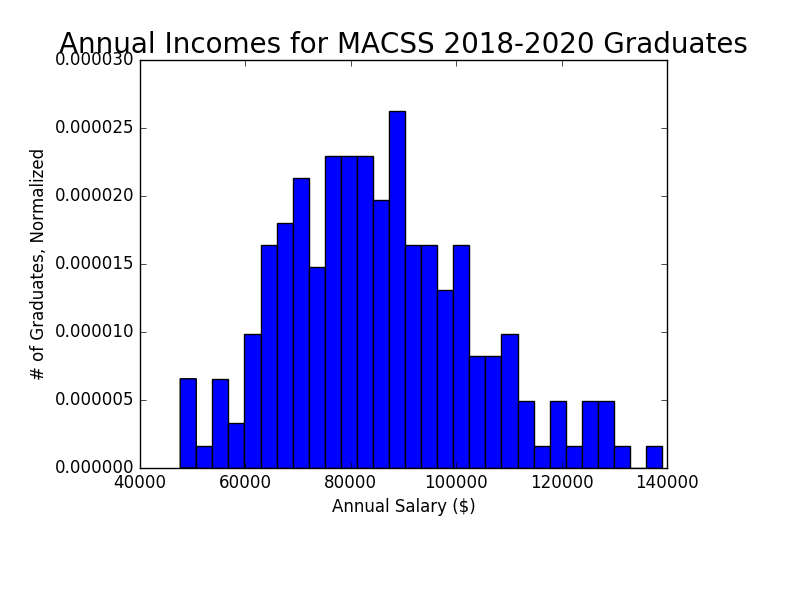
\includegraphics{PS3_1a.png}}}
\end{figure}

\noindent\newline\textbf{Part 1b.} Given the lognormal probability distribution function as the model and data from the incomes.txt file, the Generalized Method of Moments (GMM) method was used to estimate the parameters $\mu$ and $\sigma$, taking the average income and the standard deviation for the two moments. Method 'SLSQP' was used for the optimization. The identity matrix was used for the Weighting matrix. The initial parameters used, the estimated parameters obtained using GMM ($\mu_{GMM1b}$ and $\sig_{GMM1b}$), the data and model moments at the estimated parameters, as well as the value of the GMM criterion function are reported in the table below. The model with estimated parameters has been plotted on the histogram from Part 1a, below. A comparison of the data and model moments at the estimated parameters suggests that the estimated parameters returned do not offer a good fit for the data: the mean of the data and model moments are considerably dissimilar, and the graph of the model with estimated parameters $\mu_{GMM1b}$ and $\sig_{GMM1b}$ shows a visibly poor fit with the data plotted in histogram format.

\begin{center}
\resizebox{\textwidth}{!}{%
    \caption{GMM method estimates with method 'SLSQP'}
    \begin{tabular}{ | l | l |}
    \hline
    Variable & Value  \\ \hline
    $\mu_{initial}$ & 11.3 \\ \hline
    $\sig_{initial}$ & 0.68  \\ \hline
    $\mu_{GMM1b}$ & 11.3314417737  \\ \hline
    $\sig_{GMM1b}$ & 0.211676166182 \\ \hline
    Data Moments(mean, std dev) & [85276.8236063, 17992.542128] \\ \hline
    Model Moments(mean, std dev)  & [35096.21330019995, 22415.7480359] \\ \hline
    Value of GMM criterion function  &  0.4067011 \\ \hline
    \end{tabular}}
\end{center}

\begin{figure}[htb]\centering\captionsetup{width=4.0in}
  \caption{\textbf{Histogram of Annual Incomes for MACS 2018-2020 Graduates, Normalized, Part 1b}}\label{FigPS3_1b}
  \fbox{\resizebox{4.0in}{3.0in}{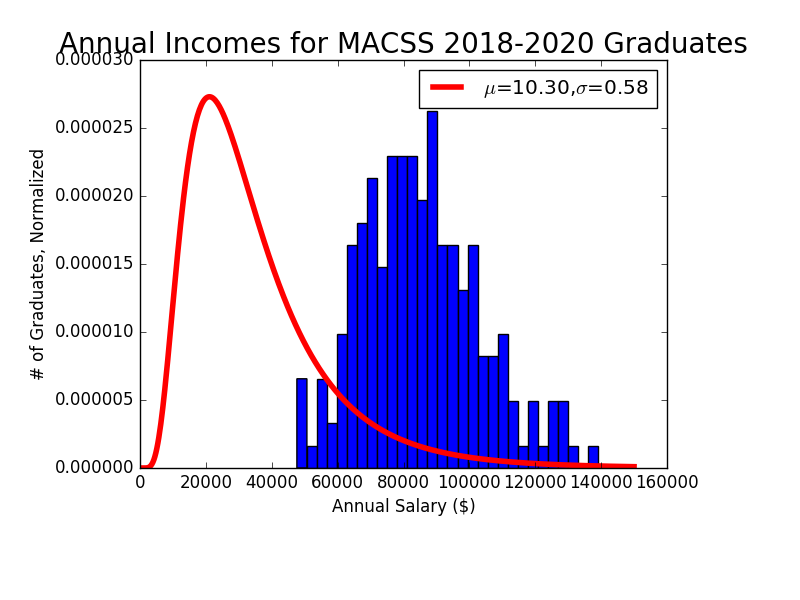
\includegraphics{PS3_1b.png}}}
\end{figure}

\noindent\newline\textbf{Part 1c.} The two-step GMM estimator was performed with the estimated parameters from Part 1b, this time, taking the inverse of the variance covariance matrix from Part1b as the optimal weighting matrix.  Method 'SLSQP' was used for the optimization. The initial parameters used, the estimated parameters obtained using two-step GMM ($\mu_{GMM1c}$ and $\sig_{GMM1c}$), the data and model moments at the estimated parameters, as well as the value of the two-step GMM criterion function are reported in the table below. The model with estimated parameters has been plotted on the histogram from Part 1a-b, below. A comparison of the data and model moments at the estimated parameters suggests that the estimated parameters returned do not offer a good fit for the data: the mean of the data and model moments are even more dissimilar than in Part 1b, and the graph of the model with estimated parameters $\mu_{GMM1c}$ and $\sig_{GMM1c}$ shows an even worse fit with the data, compared to the model generated in Part 1b.

\begin{center}
\resizebox{\textwidth}{!}{%
    \caption{2-step GMM method estimates with method 'SLSQP'}
    \begin{tabular}{ | l | l |}
    \hline
    Variable & Value  \\ \hline
    $\mu_{initial}$ & 11.3314417737  \\ \hline
    $\sig_{initial}$ & 0.211676166182  \\ \hline
    $\mu_{GMM1c}$ &  8.3267560182 \\ \hline
    $\sig_{GMM1c}$  &  3.99026484077e-09 \\ \hline
    Data Moments(mean, std dev) & [85276.8236063, 17992.542128] \\ \hline
    Model Moments(mean, std dev)  & [0,0] \\ \hline
    Value of GMM criterion function  &   141.93019032 \\ \hline
    \end{tabular}}
\end{center}

\begin{figure}[htb]\centering\captionsetup{width=4.0in}
  \caption{\textbf{Histogram of Annual Incomes for MACS 2018-2020 Graduates, Normalized, Part 1c}}\label{FigPS3_1c}
  \fbox{\resizebox{4.0in}{3.0in}{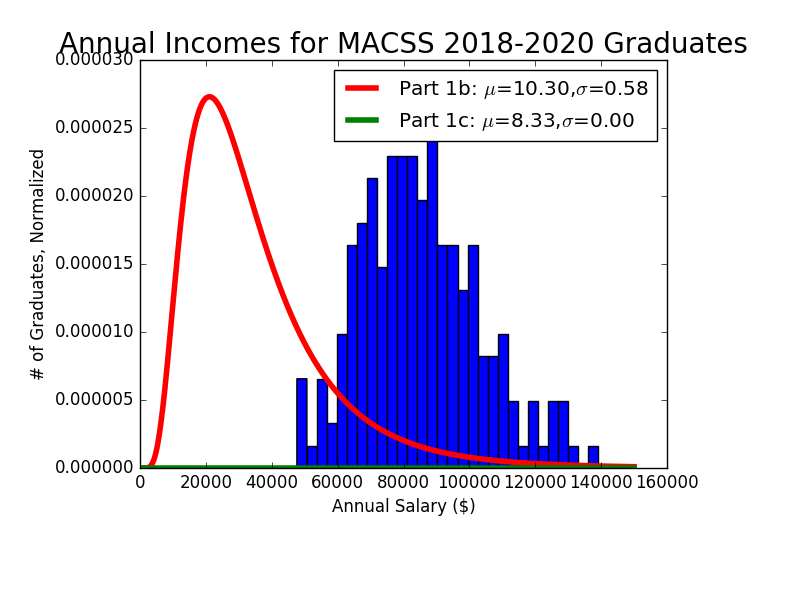
\includegraphics{PS3_1c.png}}}
\end{figure}

\noindent\newline\textbf{Part 1d.} Using the same lognormal probability function as the model, GMM was performed anew with a different set of moments. The three moments (mom\textsubscript{1}, mom\textsubscript{2}, mom\textsubscript{3}) used assigned, respectively: percentage of individuals earning less than \$75,000, percentage of individuals earning between \$75,000 (inclusive) and \$100,000 (exclusive), and percentage of individuals earning greater than \$100,000 (inclusive). Method 'SLSQP' was used for the optimization. The identity matrix was used for the Weighting matrix. The initial parameters used, the estimated parameters obtained using GMM ($\mu_{GMM1d}$ and $\sig_{GMM1d}$), the data and model moments at the estimated parameters, as well as the value of the GMM criterion function are reported in the table below. The model with estimated parameters has been plotted on the histogram from Part 1a-c, below. A comparison of the data and model moments at the estimated parameters suggests that the estimated parameters returned using these three moments offer a reasonably good fit for the data, as indicated both by the close agreement between the data and model moments, as well as the visually good fit observed in the histogram and models plotted, below. Indeed, this method has returned the model parameters that appear to best fit the data.

\begin{center}
\resizebox{\textwidth}{!}{%
    \caption{GMM method estimates, alternate moments with method 'SLSQP'}
    \begin{tabular}{ | l | l |}
    \hline
    Variable & Value  \\ \hline
    $\mu_{initial}$ & 11.3  \\ \hline
    $\sig_{initial}$ & 0.68  \\ \hline
    $\mu_{GMM1d}$ &  11.3355446226 \\ \hline
    $\sig_{GMM1d}$ &  0.210626812956 \\ \hline
    Data Moments(mom\textsubscript{1}, mom\textsubscript{2}, mom\textsubscript{3}) & [0.3, 0.5, 0.2] \\ \hline
    Model Moments(mom\textsubscript{1}, mom\textsubscript{2}, mom\textsubscript{3})  & [0.3000007042684152, 0.49999860772515586, 0.2000006880064293] \\ \hline
    Value of GMM criterion function  &  2.50985826e-07 \\ \hline
    \end{tabular}}
\end{center}

\begin{figure}[htb]\centering\captionsetup{width=4.0in}
  \caption{\textbf{Histogram of Annual Incomes for MACS 2018-2020 Graduates, Normalized, Part 1d}}\label{FigPS3_1d}
  \fbox{\resizebox{4.0in}{3.0in}{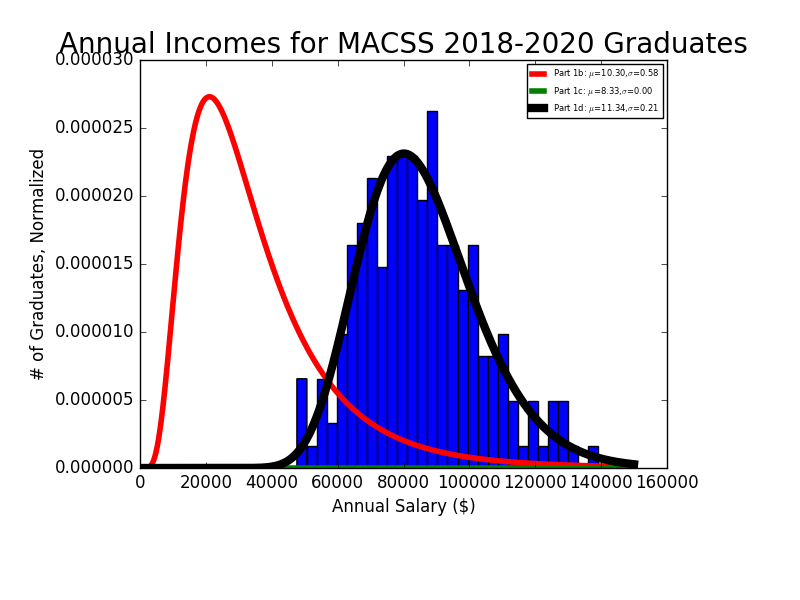
\includegraphics{PS3_1d.png}}}
\end{figure}

\noindent\newline\textbf{Part 1e.} The two-step GMM estimator was performed with the estimated parameters from Part 1d, this time, taking the inverse of the variance covariance matrix from Part1d as the optimal weighting matrix.  Method 'SLSQP' failed, so method 'L-BFGS-B' was used for the optimization instead. The initial parameters used, the estimated parameters obtained using two-step GMM ($\mu_{GMM1e}$ and $\sig_{GMM1e}$), the data and model moments at the estimated parameters, as well as the value of the two-step GMM criterion function are reported in the table below. The model with estimated parameters has been plotted on the histogram from Part 1a-d, below. The two-step GMM estimator effectively returned the same estimated parameter values as that in Part 1d.

\begin{center}
\resizebox{\textwidth}{!}{%
    \caption{2-step GMM method estimates, alternate moments with method 'L-BFGS-B'}
    \begin{tabular}{ | l | l |}
    \hline
    Variable & Value  \\ \hline
    $\mu_{initial}$ & 11.3  \\ \hline
    $\sig_{initial}$ & 0.68  \\ \hline
    $\mu_{GMM1e}$ &  11.3355417879 \\ \hline
    $\sig_{GMM1e}$ &  0.210626759407 \\ \hline
    Data Moments(mom\textsubscript{1}, mom\textsubscript{2}, mom\textsubscript{3}) & [0.3, 0.5, 0.2] \\ \hline
    Model Moments(mom\textsubscript{1}, mom\textsubscript{2}, mom\textsubscript{3})  & [0.30000533738948193, 0.49999780237528935, 0.19999686023522892] \\ \hline
    Value of 2-step GMM criterion function  &  7.82585544e-08 \\ \hline
    \end{tabular}}
\end{center}

\begin{figure}[htb]\centering\captionsetup{width=4.0in}
  \caption{\textbf{Histogram of Annual Incomes for MACS 2018-2020 Graduates, Normalized, Part 1e}}\label{FigPS3_1e}
  \fbox{\resizebox{4.0in}{3.0in}{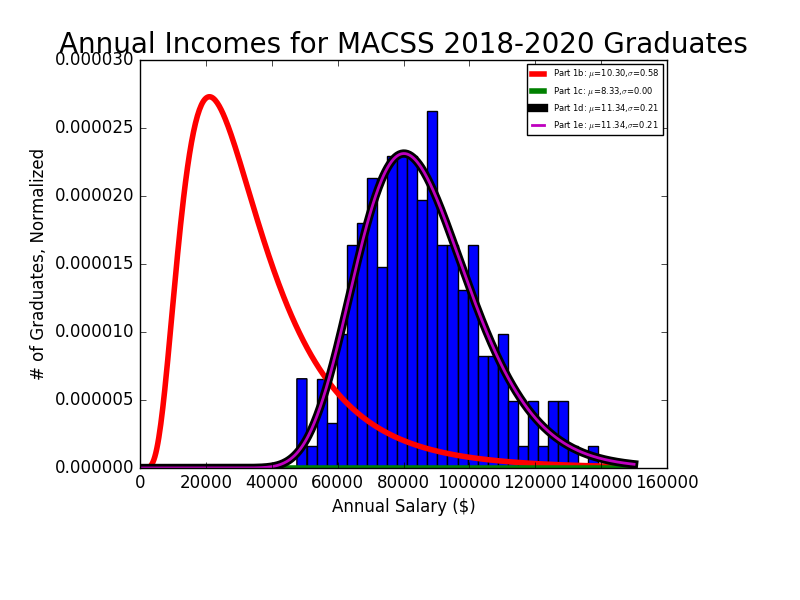
\includegraphics{PS3_1e.png}}}
\end{figure}

\noindent\newline\textbf{Part 1f.} The parameter estimations obtained from GMM from Parts 1d and 1e returned the best fit for the data (Parts 1d and 1e returned the same parameter estimates). The model and data moments from Parts 1d and 1e at the estimated parameters were nearly identical, while the model and data moments at the estimated parameters from Parts 1b and 1c were very dissimilar. This is one indication that the "distance" between the model and data moments was better minimized using the three moments used in Parts 1d and 1e than the two moments used in Parts 1b and 1c. Another indication of the better fit which the estimated parameters from Parts 1d and 1e provided is seen visually by the graphs in Part 1e. The estimated parameters from Parts 1d and 1e return a model with a closer fit to the actual histogram of the data, with the bulk of the data contained under the curve, unlike the curves produced from the models in Parts 1a and 1b. If a best estimation must be selected between the results from Part 1d and 1e, the parameter estimations from Part 1e could be considered as having a better fit to the data than the estimations from Part 1d due to the smaller (more minimized) value of the GMM criterion function obtained using the two-step weighting matrix in Part 1e than in Part 1d. This effectively tells us that the error vector, and thus by inference also, the difference between the data and model as summarized by the data and model moments, has been more effectively reduced in Part 1e than in Part 1d.

\noindent\newline\textbf{Problem 2}
\noindent\newline\textbf{Part 2a.} GMM was used to estimated the parameters for a linear regression, using the data from sick.txt file and the 200 values of the variable \textbf{\textit{sick\textsubscript{i}}} for the data moment, calculating the model moments using the linear regression model below. Method 'SLSQP' was used for the optimization. The identity matrix was used for the Weighting matrix. The error vector was calculated using the simple difference (not the percent difference) of the data moments from the model moments. The initial parameters used, the estimated parameters obtained using GMM ($\beta_{0_GMM}$, $\beta_{1_GMM}$, $\beta_{2_GMM}$, $\beta_{3_GMM}$) and the value of the GMM criterion function are reported in the table below. 

\begin{equation}
sick\textsubscript{i} = \beta_{0} + \beta_{1}sick\textsubscript{i} + \beta_{2}children\textsubscript{i}  + \beta_{3}tempwinter\textsubscript{i} + \epsilon_{1}
\end{equation}

\begin{center}
\resizebox{\textwidth}{!}{%
    \caption{GMM paramter estimates with method 'SLSQP'}
    \begin{tabular}{ | l | l | l |}
    \hline
    Variable & Value \\ \hline
    $\beta_{0_GMM}$ &  0.25164447235  \\ \hline
    $\beta_{1_GMM}$ &  0.0129333849031  \\ \hline
    $\beta_{2_GMM}$ &  0.400501883538 \\ \hline
    $\beta_{3_GMM}$ & -0.00999165469161 \\ \hline
    Value of 2-step GMM criterion function  &  0.00182128989133 \\ \hline
    \end{tabular}}
\end{center}

\end{document}

